\chapter{La placa \dato{pcbVersion}}\label{cap:pcb}

La placa reparte los 12~V de la fuente hacia las dos caras y hacia el regulador, protege cada salida con un fusible y lleva la ESP32-S3 que genera la señal de datos. El proyecto de KiCad está en \texttt{Documents/KiCad/Projects/PCB\_V2/} (\texttt{PCB\_V2.kicad\_pro}); los Gerbers de fabricación están en \texttt{gerber.zip} de esa misma carpeta y se incluyen en la carpeta de entregables.

\begin{figure}[H]\centering
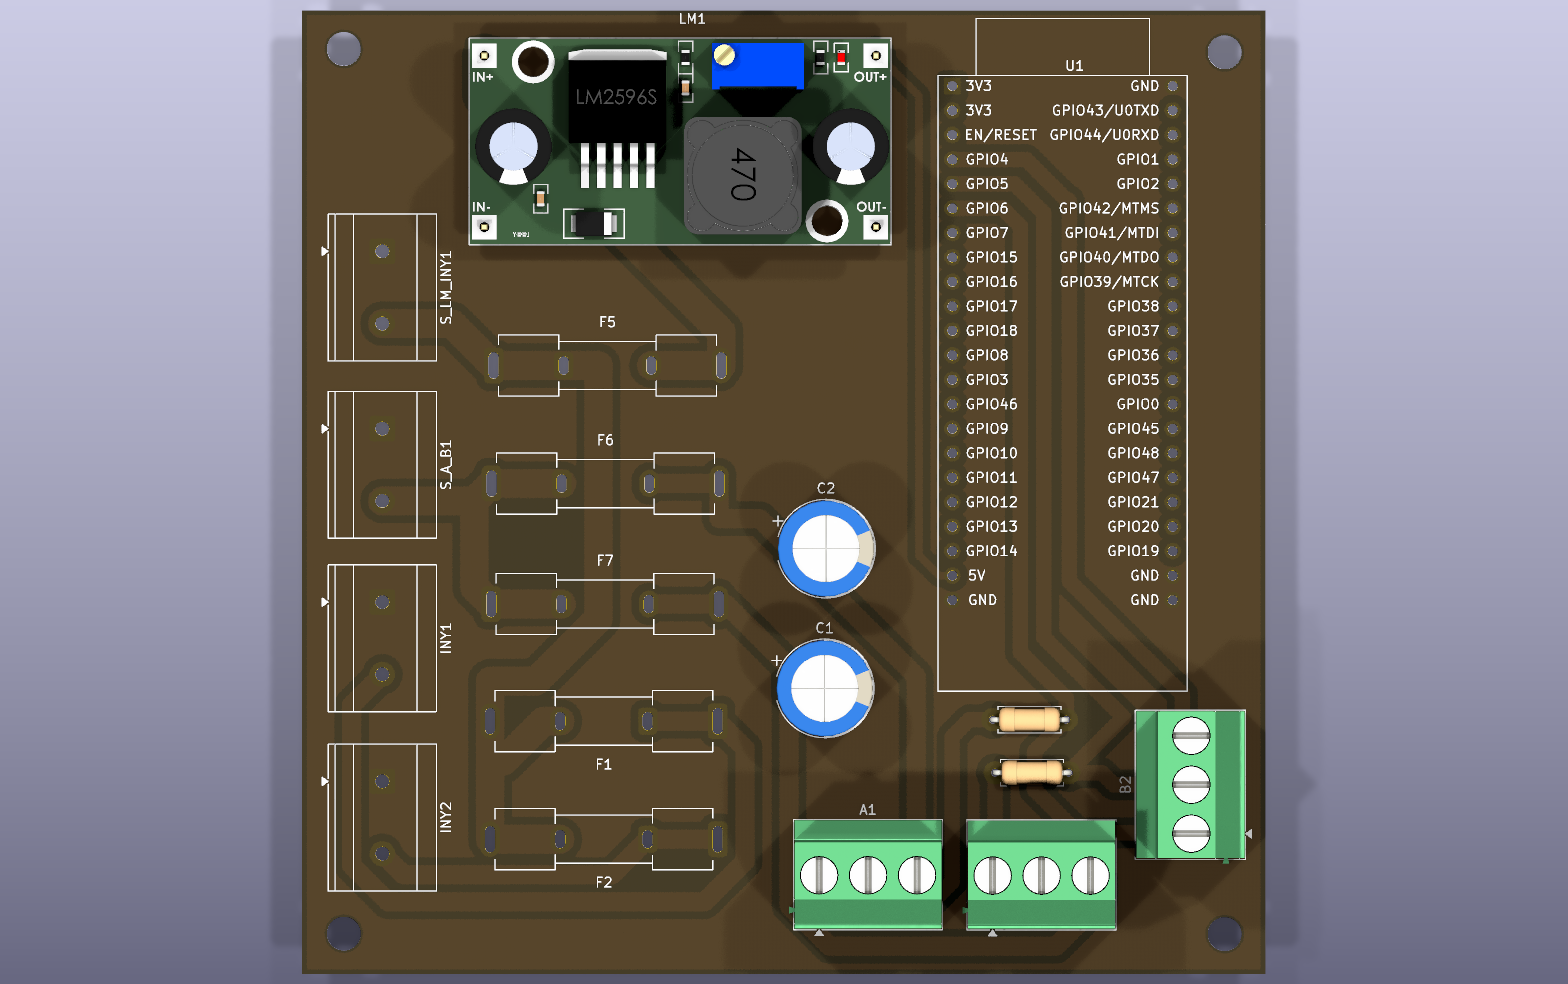
\includegraphics[width=0.92\linewidth]{img/pcb/3d-superior.png}
\caption{Vista superior generada desde KiCad.}\label{fig:3d-superior}
\end{figure}

\begin{figure}[H]\centering
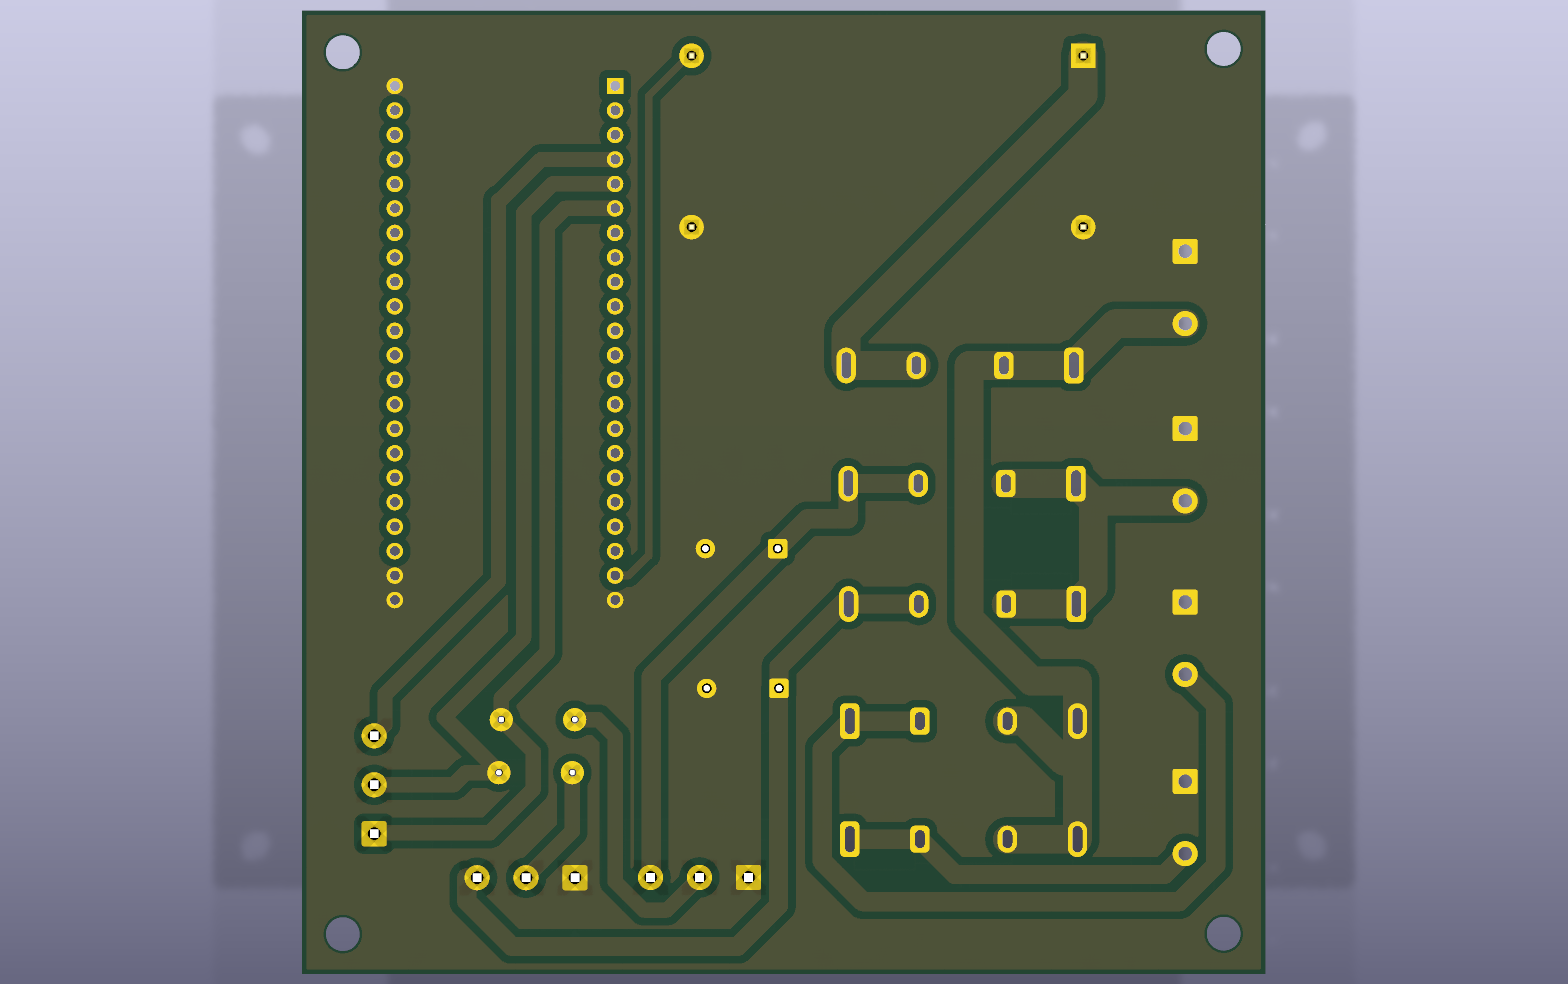
\includegraphics[width=0.92\linewidth]{img/pcb/3d-inferior.png}
\caption{Vista inferior generada desde KiCad.}
\end{figure}

\foto{placa-superior}{Placa del poste que funciona, vista desde arriba. A la izquierda, la ESP32-S3 en su placa de borneras, unida por cables a la bornera de datos B2 (arriba a la izquierda) y a la de 5~V. Arriba, las borneras A1 y B1 de las caras; a la derecha, los cinco portafusibles y las cuatro borneras de 12~V; abajo, el regulador LM2596.}{0.9}
\foto{placa-inferior}{Cara de cobre de la placa del poste que funciona, vista desde abajo: pistas y soldaduras sobre el plano de tierra.}{0.6}

\nota{La placa de las fotos es la del poste que funciona. No lleva la ESP32 soldada (va en una placa de borneras aparte) y tiene una bornera de 2 polos para los 5~V de la ESP32 que la \dato{pcbVersion} no tiene. Las vistas de KiCad de arriba son las de la \dato{pcbVersion}.}

\section{Borneras y conexiones}

Las conexiones salen del esquema de KiCad (redes entre paréntesis). El número de borne se cuenta según la serigrafía de la placa.

\begin{longtable}{@{}p{0.17\linewidth} p{0.33\linewidth} p{0.43\linewidth}@{}}
\toprule
\textbf{Bornera} & \textbf{Bornes} & \textbf{Función} \\ \midrule \endhead
S\_LM\_INY1 & 1 GND · 2 +12~V (\texttt{+12V\_INY}) & Entrada de 12~V para el regulador LM2596 y para las dos salidas de inyección. \\
S\_A\_B1 & 1 GND · 2 +12~V (\texttt{+12V\_CARAS}) & Entrada de 12~V para las caras; se reparte por F6 y F7. \\
A1 & 1 GND · 2 datos (\texttt{D1}) · 3 +12~V (\texttt{+12V\_A}) & Cara A: alimentación por F6 y datos desde R1. \\
B1 & 1 GND · 2 datos (\texttt{D2}) · 3 +12~V (\texttt{+12V\_B}) & Cara B: alimentación por F7 y datos desde R2. \\
INY1 & 1 GND · 2 +12~V (\texttt{INY1}) & Inyección de 12~V por F1, para el extremo lejano de una cara. \\
INY2 & 1 GND · 2 +12~V (\texttt{INY2}) & Inyección de 12~V por F2, para el extremo lejano de la otra cara. \\
B2 & 1 \texttt{GPIO\_A} · 2 \texttt{GPIO\_B} · 3 \texttt{GPIO\_C} & Señales de datos de la ESP32 antes de las resistencias (medición y señal adicional). \\
\bottomrule
\end{longtable}

\section{Otros componentes}

\begin{description}[leftmargin=0pt]
\item[LM1 · LM2596] Módulo reductor que baja los 12~V a \dato{reguladorSalida} para la ESP32 (red \texttt{+5V\_ESP}, pin 21 «5V» del módulo). Se ajusta con su potenciómetro antes de poner la ESP32 (capítulo~\ref{cap:ensamble}).
\item[U1 · ESP32-S3] Se conecta por su pin 5V (21) y sus pines GND (22, 23, 24 y 44). La zona de la antena no tiene cobre en ninguna de las dos caras de la placa.
\item[R1 y R2] Resistencias de 330~Ω en serie entre la ESP32 y la línea de datos de cada cara (\texttt{GPIO\_A}→\texttt{D1}, \texttt{GPIO\_B}→\texttt{D2}).
\item[C1 y C2] Condensadores electrolíticos de 1000~µF en la alimentación de cada cara (C2 en \texttt{+12V\_A}, C1 en \texttt{+12V\_B}). Respeta la polaridad.
\end{description}

\section{Fusibles}

\begin{tabularx}{\linewidth}{@{}l l X@{}}
\toprule
\textbf{Fusible} & \textbf{Protege} & \textbf{Estado} \\ \midrule
F1 & Inyección INY1 & Activo. \\
F2 & Inyección INY2 & Activo. \\
F5 & Regulador LM2596 (\texttt{+12V\_LM}) & Activo desde la corrección del 18-11-2026 (ver abajo). En placas fabricadas antes, no protege. \\
F6 & Cara A (\texttt{+12V\_A}) & Activo. \\
F7 & Cara B (\texttt{+12V\_B}) & Activo. \\
\bottomrule
\end{tabularx}

\advertencia{\textbf{F5 en placas fabricadas antes del 18-11-2026:} sus dos patas estaban en la misma red (\texttt{+12V\_INY}) en el esquema, y en la placa una pista las unía. Aunque le pongas un fusible, el regulador queda sin protección. En esas placas, protege la línea con un fusible externo en el cable que sale de la fuente (capítulo~\ref{cap:cableado}), o corta la pista de la cara inferior entre la pata 1 de F5 (la del lado de S\_LM\_INY1) y su pata 2, y comprueba con el multímetro que ya no hay continuidad entre las dos patas sin el fusible puesto.}

\paragraph{Corrección de F5.} En el esquema, el lado de F5 que va al LM2596 se llama ahora \texttt{+12V\_LM}. En la placa se quitó el tramo de pista que unía las dos patas de F5, y la pata 2 de F5, la pista y la entrada del LM2596 pasaron a \texttt{+12V\_LM}. Así, cada ramal de la entrada S\_LM\_INY1 tiene su fusible: F5 el regulador, F1 la inyección INY1 y F2 la inyección INY2. Tras el cambio, el ERC no tiene errores y el DRC no tiene errores, conexiones pendientes ni diferencias con el esquema. Los Gerber y los archivos de taladro se volvieron a exportar; los anteriores quedaron en \texttt{respaldo-antes-F5-2026-11-18/} dentro del proyecto de KiCad.

\nota{Los portafusibles Keystone 3512P son abiertos: no tienen sellado contra agua, polvo ni condensación. Solo sirven dentro de una caja estanca.}

\section{Estado de verificación del diseño}

El chequeo eléctrico del esquema (ERC) no tiene errores. El chequeo de la placa (DRC) no tiene conexiones pendientes ni errores de separación entre pistas; quedan 10 avisos heredados de la versión anterior (8 de serigrafía sobre cobre y 2 de huellas de resistencias modificadas respecto a la biblioteca). Revísalos si se manda a fabricar un lote nuevo.
